\subsection{Тестирование производительности алгоритмов\label{tesing}}

Проведём тестирование производительности некоторых алгоритмов генерации ансамблей. 

Следующие параметры влияют на время генерации случайного ансамбля:
\begin{enumerate}
    \item 
        Количество элементов
    \item 
        Начальная конфигурация элементов. В зависимости от того, как расположены элементы в начальном положении, меняется скорость генерации случайного ансамбля. Если генерация начинается с расположения элементов по узлам сетки, то скорость получения случайно распределенного ансамбля будет больше, чем если генерация начинается с формации плотнейшей упаковки. Данный аспект вызван тем, что генерация положений для плотнейшей упаковки сложнее чем для расположения в узлах сетки. Также стоит учесть, что при генерации из формации плотнейшей упаковки также добавляется шаг растягивания упаковки на всю ширину пространства.
    \item 
        Количество перемешиваний для достижения равномерного распределения (актуально для методов генерации начинающих с какой-либо определенной формации).
    
\end{enumerate}

\renewcommand{\imgsubdir}{speed_analysis}
\begin{figure}[h!]
    \centering
    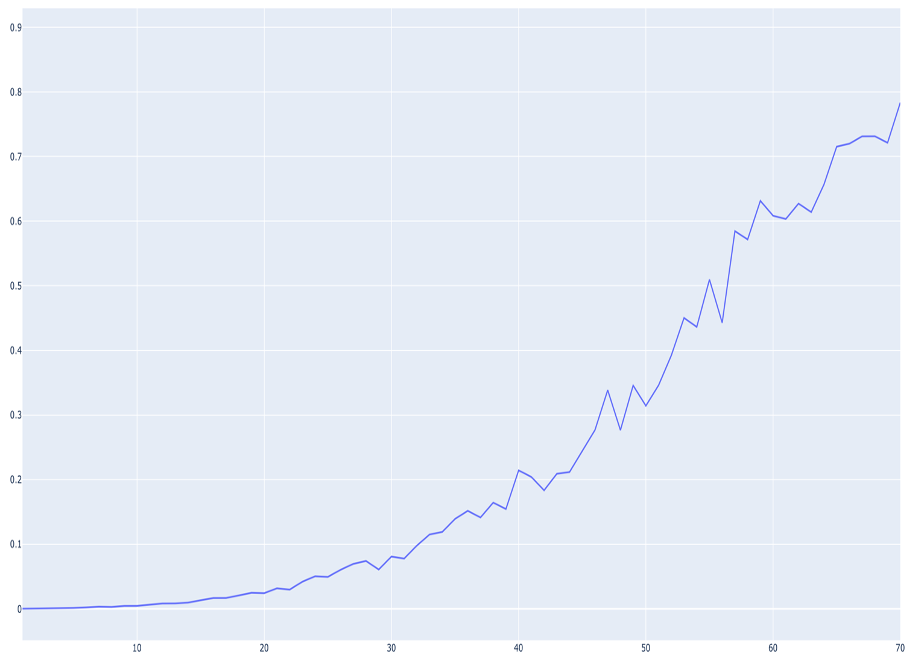
\includegraphics{\imgdir/\imgsubdir/t_by_circle_count.png}
    \caption{Зависимость времени генерации области от количества окружностей}
    \label{fig:my_label}
\end{figure}

\begin{figure}[h]
    \centering
    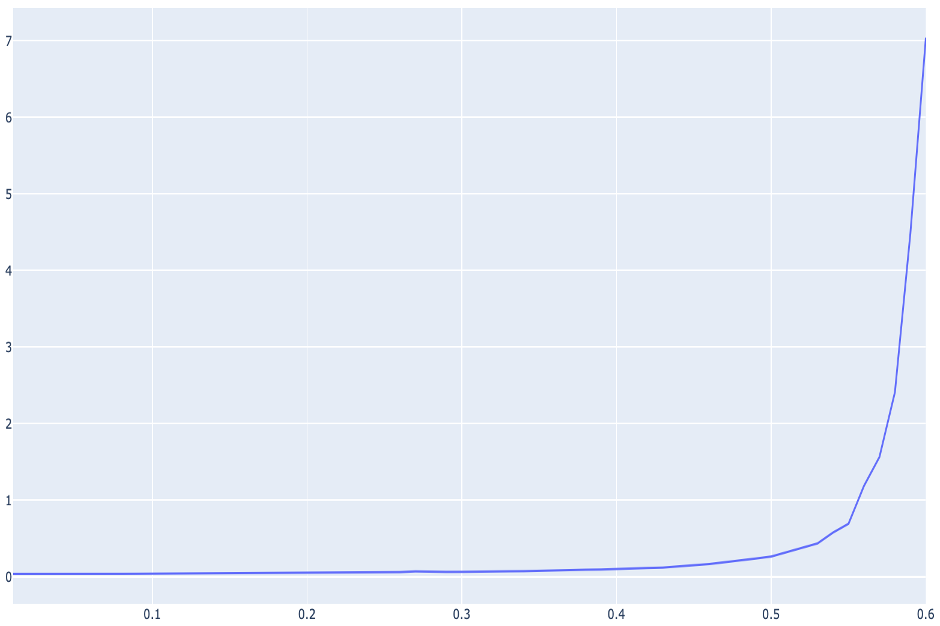
\includegraphics{\imgdir/\imgsubdir/t_by_rho.png}
    \caption{Зависимость времени генерации области от процента заполненности}
    \label{fig:my_label}
\end{figure}

